\documentclass[11pt,fleqn]{article} 
\usepackage[margin=0.8in, head=0.8in]{geometry} 
\usepackage{amsmath, amssymb, amsthm}
\usepackage{fancyhdr} 
\usepackage{palatino, url, multicol}
\usepackage{graphicx,latexsym} 
\usepackage[all]{xy}
\usepackage{polynom} 
\usepackage{pdfsync}
\usepackage{enumerate, enumitem}
\usepackage{framed}
\usepackage{setspace}
\usepackage{array,tikz,xcolor, pgfplots}
\pagestyle{fancy} 
\lfoot{UAF Calculus 1}
\rfoot{\S 2.2 }

\usetikzlibrary{calc}
\pgfplotsset{compat=1.6}

\pgfplotsset{soldot/.style={color=black,only marks,mark=*}} \pgfplotsset{holdot/.style={color=black,fill=white,only marks,mark=*}}

\begin{document}
\setlength{\parindent}{0cm}
\renewcommand{\headrulewidth}{0pt}
\newcommand{\blank}[1]{\rule{#1}{0.75pt}}
\renewcommand{\d}{\displaystyle}


\vspace*{-1in}
\begin{center}
   \sc{Lecture Notes: \S 2.2 }
\end{center}

\begin{enumerate}
\item The function $f(x)$ is graphed below. Use the graph to fill in the blanks.

\begin{multicols}{2}
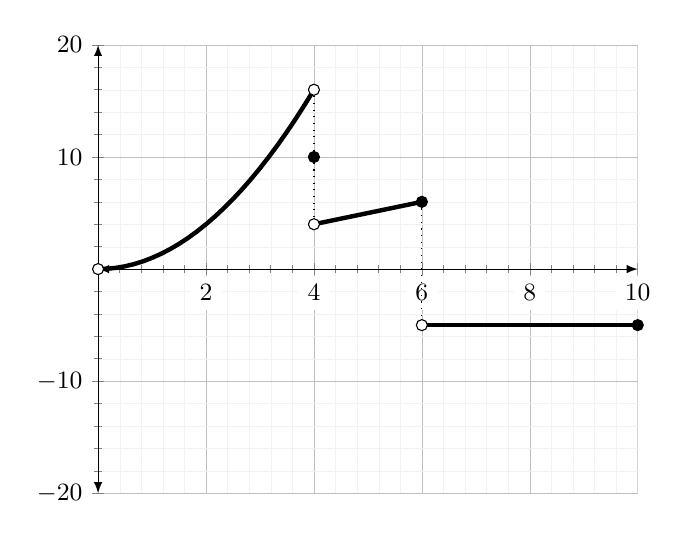
\begin{tikzpicture}[scale=1]
\begin{axis}[grid style={line width=.1pt, draw=gray!10},grid=both,major grid style={line width=.2pt,draw=gray!50},
    xmin=0,xmax=10,
    ymin=-20,ymax=20,
    xtick={},ytick={},
    minor tick num=4,
    enlargelimits={abs=0},
    ticklabel style={font=\small,fill=white},
    axis lines=middle,
    axis line style={latex-latex},
    xlabel style={at={(ticklabel* cs:1)},anchor=north west},
    ylabel style={at={(ticklabel* cs:1)},anchor=south west}
]
\addplot[domain=0:4,ultra thick] {x*x};
\addplot[domain=4:6,ultra thick] {x};
\addplot[domain=6:10,ultra thick] {-5};
\draw[dotted] (axis cs:4,16) -- (axis cs:4,4);
\draw[dotted] (axis cs:6,6) -- (axis cs:6,-5);
\addplot[holdot] coordinates{(0,0)(4,16)(4,4)(6,-5)};
\addplot[soldot] coordinates{(4,10)(6,6)(10,-5)};
\end{axis}
\end{tikzpicture}
\begin{enumerate}
\item $\d{\lim_{x \to 4^-} f(x) = \underline{\hspace{2cm}} }$\\
\item $\d{\lim_{x \to 4^+} f(x) = \underline{\hspace{2cm}} }$\\
\item $\d{\lim_{x \to 4} f(x) = \underline{\hspace{2cm}} }$\\
\item $f(4)= \underline{\hspace{2cm}}$\\


\item $\d{\lim_{x \to 6^-} f(x) = \underline{\hspace{2cm}} }$\\
\item $\d{\lim_{x \to 6^+} f(x) = \underline{\hspace{2cm}} }$\\
\item $\d{\lim_{x \to 6} f(x) = \underline{\hspace{2cm}} }$\\
\item $f(6)= \underline{\hspace{2cm}}$\\
\item $\d{\lim_{x \to 8} f(x) = \underline{\hspace{2cm}} }$\\
\item $f(8)= \underline{\hspace{2cm}}$\\
\end{enumerate}
\end{multicols}

\item The function $g(x)$ is graphed below. Use the graph to fill in the blanks.

\begin{multicols}{2}
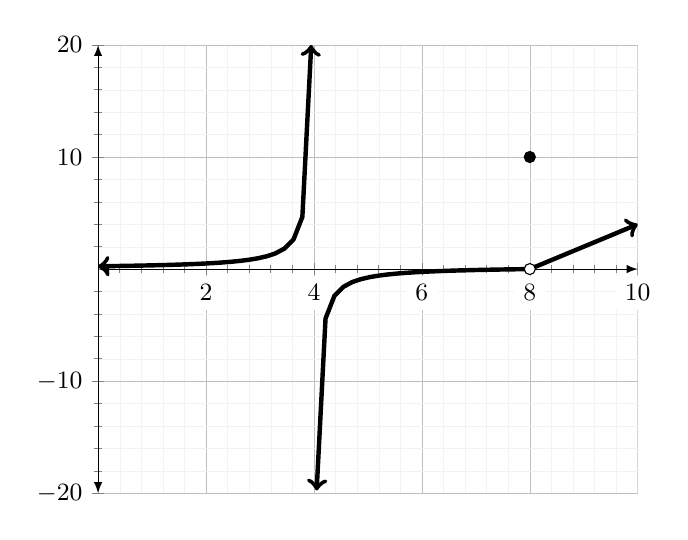
\begin{tikzpicture}[scale=1]
\begin{axis}[grid style={line width=.1pt, draw=gray!10},grid=both,major grid style={line width=.2pt,draw=gray!50},
    xmin=0,xmax=10,
    ymin=-20,ymax=20,
    xtick={},ytick={},
    minor tick num=4,
    enlargelimits={abs=0},
    ticklabel style={font=\small,fill=white},
    axis lines=middle,
    axis line style={latex-latex},
    xlabel style={at={(ticklabel* cs:1)},anchor=north west},
    ylabel style={at={(ticklabel* cs:1)},anchor=south west}
]

\addplot[<->,domain=0:3.95,ultra thick] {(4-x)^(-1)};
\addplot[<-,domain=4.05:8,ultra thick] {(4-x)^(-1)+0.25};
\addplot[->,domain=8:10,ultra thick] {2*x-16};
%\draw[dotted] (axis cs:4,16) -- (axis cs:4,4);
%\draw[dotted] (axis cs:6,6) -- (axis cs:6,-5);
\addplot[soldot] coordinates{(8,10)};
\addplot[holdot] coordinates{(8,0)};
\end{axis}
\end{tikzpicture}
\columnbreak
\begin{enumerate}
\item $\d{\lim_{x \to 4^-} g(x) = \underline{\hspace{2cm}} }$
\item $\d{\lim_{x \to 4^+} g(x) = \underline{\hspace{2cm}} }$
\item $\d{\lim_{x \to 4} g(x) = \underline{\hspace{2cm}} }$
\item $g(4)= \underline{\hspace{2cm}}$
\item $\d{\lim_{x \to 8} g(x) = \underline{\hspace{2cm}} }$
\item $g(8)= \underline{\hspace{2cm}}$
\end{enumerate}
\end{multicols}

Write the equation of any vertical asymptotes:\\
\newpage

\item Evaluate the limits below by graphing $f(x)=\begin{cases} x+1 & x < 0 \\ 
x -1 & 0 \leq x < 2 \\
1+\sqrt{x-2}& 2<x \\
\end{cases}$
\vspace{2in}
\begin{enumerate}
\item $\d{\lim_{x \to 0} f(x)}$
\vspace{.7in}
\item $\d{\lim_{x \to 2} f(x)}$
\vspace{.7in}
\item For which values $a$ does $\lim_{x \to a} f(x)$ exist?
\end{enumerate}
\end{enumerate}
\end{document}
\newpage
\item Use a calculator and a table of values to determine the limit: $\d{\lim_{x \to 0^+} \left(\frac{1}{x} - \ln (x)\right)}.$
\vfill
\item Sketch the graph of an example of a function $f$ that satisfies \emph{all} of the given conditions.
\begin{enumerate}
\item $\d{\lim_{x \to 0}f(x)}=1$
\item $\d{\lim_{x \to 3^-} f(x)= -2}$
\item $\d{\lim_{x \to 3^+} f(x)= 4}$
\item $f(0)=2$

\item $f(3)=1$

\item $\d{\lim_{x \to -1^+}f(x)= \infty}$
\end{enumerate}
\end{enumerate}

\end{document}